\documentclass{beamer}
\mode<presentation>
\usepackage{amsmath}
\usepackage{amssymb}
\usepackage{adjustbox}
\usepackage{subcaption}
\usepackage{enumitem}
\usepackage{multicol}
\usepackage{mathtools}
\usepackage{listings}
\usepackage{url}
\usepackage{circuitikz}
\def\UrlBreaks{\do\/\do-}
\usetheme{Boadilla}
\usecolortheme{seahorse}
\setbeamertemplate{footline}
{
  \leavevmode%
  \hbox{%
  \begin{beamercolorbox}[wd=\paperwidth,ht=2.25ex,dp=1ex,right]{author in head/foot}%
    \insertframenumber{} / \inserttotalframenumber\hspace*{2ex} 
  \end{beamercolorbox}}%
  \vskip0pt%
}
\setbeamertemplate{navigation symbols}{}
\providecommand{\nCr}[2]{\,^{#1}C_{#2}} % nCr
\providecommand{\nPr}[2]{\,^{#1}P_{#2}} % nPr
\providecommand{\mbf}{\mathbf}
\providecommand{\pr}[1]{\ensuremath{\Pr\left(#1\right)}}
\providecommand{\qfunc}[1]{\ensuremath{Q\left(#1\right)}}
\providecommand{\sbrak}[1]{\ensuremath{{}\left[#1\right]}}
\providecommand{\lsbrak}[1]{\ensuremath{{}\left[#1\right.}}
\providecommand{\rsbrak}[1]{\ensuremath{{}\left.#1\right]}}
\providecommand{\brak}[1]{\ensuremath{\left(#1\right)}}
\providecommand{\lbrak}[1]{\ensuremath{\left(#1\right.}}
\providecommand{\rbrak}[1]{\ensuremath{\left.#1\right)}}
\providecommand{\cbrak}[1]{\ensuremath{\left\{#1\right\}}}
\providecommand{\lcbrak}[1]{\ensuremath{\left\{#1\right.}}
\providecommand{\rcbrak}[1]{\ensuremath{\left.#1\right\}}}
\theoremstyle{remark}
\newtheorem{rem}{Remark}
\newcommand{\sgn}{\mathop{\mathrm{sgn}}}
\providecommand{\abs}[1]{\left\vert#1\right\vert}
\providecommand{\res}[1]{\Res\displaylimits_{#1}} 
\providecommand{\norm}[1]{\lVert#1\rVert}
\providecommand{\mtx}[1]{\mathbf{#1}}
\providecommand{\mean}[1]{E\left[ #1 \right]}
\providecommand{\fourier}{\overset{\mathcal{F}}{ \rightleftharpoons}}
%\providecommand{\hilbert}{\overset{\mathcal{H}}{ \rightleftharpoons}}
\providecommand{\system}{\overset{\mathcal{H}}{ \longleftrightarrow}}
	%\newcommand{\solution}[2]{\textbf{Solution:}{#1}}
%\newcommand{\solution}{\noindent \textbf{Solution: }}
\providecommand{\dec}[2]{\ensuremath{\overset{#1}{\underset{#2}{\gtrless}}}}
\newcommand{\myvec}[1]{\ensuremath{\begin{pmatrix}#1\end{pmatrix}}}
\let\vec\mathbf
\lstset{
%language=C,
frame=single, 
breaklines=true,
columns=fullflexible
}

\numberwithin{equation}{section}
\usebackgroundtemplate{\color{blue!10}}


\title{LU decomposition}
\author{CHARAN RONGALI \\ Electrical Engineering,\\IIT Hyderabad}
\date{\today} 

\begin{document}

\begin{frame}
\titlepage
\end{frame}

\section*{Outline}
\begin{frame}
\tableofcontents
\end{frame}

\section{Problem Statement}
\begin{frame}
\frametitle{Problem Statement}
Solve the following pairs of equations by reducing them to a pair of linear equations:
\begin{align*}
    \frac{5}{x-1} + \frac{1}{y-2} &= 2\\
    \frac{6}{x-1} - \frac{3}{y-2} &= 1
\end{align*}
\end{frame}

\section{Solution}
\subsection{Matrix Representation}
\begin{frame}
\frametitle{Matrix representation}
Let's solve this using LU decomposition. First, let's substitute:
\begin{align}
    \frac{1}{x-1} &= u\\
    \frac{1}{y-2} &= v
\end{align}

Then our equations become:
\begin{align}
    5u + v &= 2 \\
    6u - 3v &= 1
\end{align}

This can be written in matrix form as:
\begin{align}
    \myvec{5 & 1\\6 & -3}\myvec{u\\v} = \myvec{2\\1}\\
	\vec{ A}\vec{x} = \vec{L}\vec{U}\vec{x} = \vec{b}
\end{align}
\end{frame}
\subsection{Doolittle's Algorithm}
\begin{frame}
\frametitle{Doolittle's Algorithm}
This method generates the matrices \( L \) (lower triangular) and \( U \) (upper triangular) such that \( A = LU \). The elements of these matrices are calculated as follows: \\
Elements of the \( U \) Matrix:  \\
For each column \( j \):
\begin{align}
	U_{ij} &= A_{ij} \quad \text{if } i = 0, \\
	U_{ij} &= A_{ij} - \sum_{k=0}^{i-1} L_{ik} U_{kj} \quad \text{if } i > 0.
\end{align}
Elements of the \( L \) Matrix: \\
For each row \( i \):
\begin{align}
	L_{ij} &= \frac{A_{ij}}{U_{jj}} \quad \text{if } j = 0, \\
	L_{ij} &= \frac{A_{ij} - \sum_{k=0}^{j-1} L_{ik} U_{kj}}{U_{jj}} \quad \text{if } j > 0.
\end{align}
\end{frame}
\subsection{LU factorization}
\begin{frame}
\frametitle{LU factorization}
By doing the following steps and solving we get :
\begin{align}
	\vec{U}=\myvec{5 & 1\\0 & -\frac{21}{5}} \\
	\vec{ L} = \myvec{1 & 0\\\frac{6}{5} & 1}
\end{align}

Now,
\begin{align}
    A = \myvec{5 & 1\\6 & -3} = \myvec{1 & 0\\\frac{6}{5} & 1}\myvec{5 & 1\\0 & -\frac{21}{5}}
\end{align}
We can solve this using two steps:
\begin{align}
    L\vec{y} = \vec{b}\\
    U\vec{x} = \vec{y}
\end{align}
\end{frame}
\subsection{Substitution}
\begin{frame}
\frametitle{Substitution}
Using forward substitution:
\begin{align}
    \myvec{1 & 0\\\frac{6}{5} & 1}\myvec{y_1\\y_2} = \myvec{2\\1}\\
	\vec{y}= \myvec{2\\-\frac{7}{5}}
\end{align}

Now using back substitution:
\begin{align}
    \myvec{5 & 1\\0 & -\frac{21}{5}}\myvec{u\\v} = \myvec{2\\-\frac{7}{5}}\\
	\myvec{u\\v} =\myvec{\frac{1}{3}\\\frac{1}{3}} 
\end{align}

By equating this $\frac{1}{x-1} = u$ and $\frac{1}{y-2} = v$ we get
\begin{align}
    \myvec{x\\y} = \myvec{4\\5}
\end{align}
\end{frame}
\subsection{Graphical Representation}
\begin{frame}
\frametitle{Graphical Representation}
\begin{figure}[h!]
   \centering
   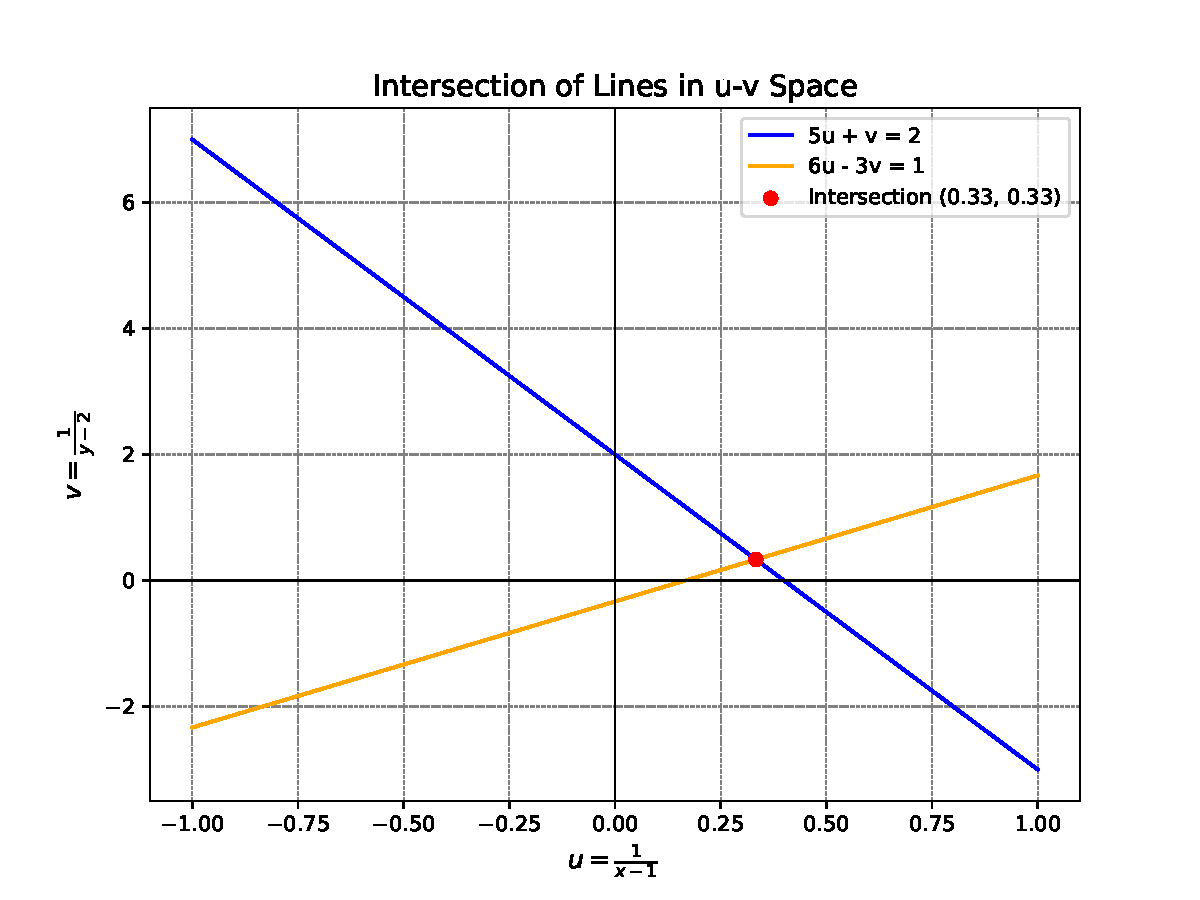
\includegraphics[width=0.9\linewidth]{figs/fig.pdf}
   \caption{Graph of the solution}
\end{figure}
\end{frame}

\end{document}

